\RequirePackage[l2tabu, orthodox]{nag}

\documentclass[
a4paper,    
% draft,       %% produce only a draft version (mark lines that need manual edition and don't show graphics)
bibliography=totoc, % add bibilography to table of contents
11pt,         %% set default font size to 11 point
DIV=14, % replace this with a larger number to get less padding around all text (or use calc for the ideal border)
parskip=half, % how much space between paragraphs. If you prefer indention instead of space between paragraphs remove it
oneside, % replace with twoside before printing
%draft, % uncomment for faster compilation
british, % language of the document
%appendixprefix=true % in case you want Appendix A written in front of appendix headings
]{scrbook}



%--------------------------- Important Packages --------------------------------

%\usepackage[ngerman]{babel}
\usepackage[american]{babel}

% required for proper characters
\usepackage[utf8]{inputenc}
\usepackage[T1]{fontenc}


% helps with equations
\usepackage{amsmath,amssymb,amstext}
\usepackage{amsthm}


\usepackage{microtype} %slightly changes letter spacing to make text fit better

\usepackage{aas_macros} % this imports the aas_macros.sty file that is required to print bibtex exported from ADS

\usepackage[svgnames]{xcolor} % allows defining colors

%------------------------------- Helpful Features ---------------------------------

% properly format 
\usepackage{siunitx}
\DeclareSIUnit{\nothing}{\relax}
\sisetup{
	per-mode=fraction, % create a fraction instead of km h^-1
%	locale=DE,
	locale=US,
	output-decimal-marker = {.}, % useful even for German
	separate-uncertainty = true,
	quotient-mode=fraction
}

%\usepackage{nicefrac}
\usepackage[autostyle=true]{csquotes} % automatically create nice quotes with \enquote{text}
\usepackage{pdflscape}  
%\usepackage{cancel}  % In case you want to cancel out some values in an equation
\usepackage{physics} % lots of shortcuts for physics equations (e.g. $\dv{a}$)

\usepackage{subcaption} % allows to nicely put two images next to each other
\usepackage{tabularx}
\usepackage{booktabs} % nicer table seperations
\usepackage{todonotes}
%----------------------------------- Style decisions -----------------------------------

\hyphenpenalty=750 % break less words than default - try different values for success
\interfootnotelinepenalty=10000 % splitting footnotes between pages is really ugly and should only be done if really necessary 
\usepackage[sc]{mathpazo} % use the Palatino font and a fitting math font

\pagestyle{headings} 
% how the header of the pages looks like
% for something nicer take a look at fancyhdr

% xcolor is already defined above

% not sure what these two do, but they definitly do something
\colorlet{bluebookmarks}{blue}
\colorlet{blueallcolors}{blue}

%----------------------------------- Bibliography ----------------------------------------


\PassOptionsToPackage{hyphens}{url}\usepackage[
	backend=biber,
	style=authoryear-comp, % choose a style from https://de.overleaf.com/learn/latex/Biblatex_citation_styles
	%sortlocale=de_AT,
	sortlocale=en_GB,
	backref=true % use if you like it -- puts a link to the page where it is cited into the bibliography
]{biblatex}

\addbibresource{bibliographie.bib}


%---------------------------------- Source Code -----------------------------------------

\usepackage[scaled=.9]{FiraMono}
\usepackage{listings}
\usepackage{scrhack} % should fix warning
\definecolor{strings}{HTML}{008000}
\definecolor{keywords}{HTML}{000080}
\definecolor{mygray}{rgb}{0.58,0,0.82}

\lstset{ %
	%	backgroundcolor=\color{white},   % choose the background color; you must add \usepackage{color} or \usepackage{xcolor}; should come as last argument
	basicstyle=\footnotesize\ttfamily,        % the size of the fonts that are used for the code
	basewidth=0.5em,
	breakatwhitespace=false,         % sets if automatic breaks should only happen at whitespace
	breaklines=true,                 % sets automatic line breaking
	captionpos=b,                    % sets the caption-position to bottom
	%	commentstyle=\color{mygreen},    % comment style
	deletekeywords={...},            % if you want to delete keywords from the given language
	escapeinside={(*}{*)},          % if you want to add LaTeX within your code
	extendedchars=true,              % lets you use non-ASCII characters; for 8-bits encodings only, does not work with UTF-8
	frame=single,	                   % adds a frame around the code
	keepspaces=true,                 % keeps spaces in text, useful for keeping indentation of code (possibly needs columns=flexible)
	keywordstyle=\color{keywords},       % keyword style
	morekeywords={*,...},            % if you want to add more keywords to the set
	numbers=none,                    % where to put the line-numbers; possible values are (none, left, right)
	numbersep=5pt,                   % how far the line-numbers are from the code
	rulecolor=\color{black},         % if not set, the frame-color may be changed on line-breaks within not-black text (e.g. comments (green here))
	showspaces=false,                % show spaces everywhere adding particular underscores; it overrides 'showstringspaces'
	showstringspaces=false,          % underline spaces within strings only
	showtabs=false,                  % show tabs within strings adding particular underscores
	stepnumber=1,                    % the step between two line-numbers. If it's 1, each line will be numbered
	stringstyle=\color{strings},     % string literal style
	tabsize=2,	                   % sets default tabsize to 2 spaces
	language=bash
}
\lstset{literate=% support Umlauts in listings
	{Ö}{{\"O}}1
	{Ä}{{\"A}}1
	{Ü}{{\"U}}1
	{ß}{{\ss}}1
	{ü}{{\"u}}1
	{ä}{{\"a}}1
	{ö}{{\"o}}1
}


%--------------------------------------- PDF output and hyperlinks ----------------------------


\usepackage{graphicx} % support graphics

\pdfcompresslevel=9 % create small files (I think it is by default when using hyperref)
\pdfsuppresswarningpagegroup=1 % https://tex.stackexchange.com/a/78020/66733


% support hyperlinks in the PDF

\usepackage[ %
colorlinks=false,   %% turn on colored links (true is better for on-screen reading, false is better for printout versions)
linkcolor = blue,
allcolors=blue,
%%% PDF-specific display options
bookmarks=true,          %% if true, generate PDF bookmarks (requires two passes of pdflatex)
bookmarksopen=false,     %% if true, show all PDF bookmarks expanded
bookmarksnumbered=false, %% if true, add the section numbers to the bookmarks
%pdfstartpage={1},        %% determines, on which page the PDF file is opened
%  pdfpagemode=None         %% None, UseOutlines (=show bookmarks), UseThumbs (show thumbnails), FullScreen
draft=false
]{hyperref}






\hypersetup{
	pdftitle={The Title of the Bachelor Thesis},
	pdfauthor={Lukas Winkler}
}
\title{The Title of the Bachelor Thesis}
\subtitle{bla bla}
\author{Lukas Winkler\footnote{\texttt{a01505981@unet.univie.ac.at}}}
%\publishers{TEST}
\date{1. August 2019}

\usepackage{lipsum}  % just for lorem ipsum
\newcommand{\blabla}{Bla bla bla}

\begin{document}
	
\maketitle

\tableofcontents

\chapter{Introduction}\label{introduction}


Here comes some short science explanation about how planets form and water is transported.
\lipsum[1]

\section{The perfect merging assumption}

To better understand how this process works, large n-body simulations over the lifetime of the solar systems have been conducted.\todo{give an example} Most of these neglect the physical details of collisions when two bodies collide for simplicity and instead assume that a perfect merging occurs. So all the mass of the two progenitor bodies and especially all of their water (ice) is retained in the newly created body. Obviously this is a simplification as in real collisions perfect merging is very rare and most of the time either partial accretion or a hit-and-run encounter occurs. (\cite{CollisionTypes}) Therefore the amount of water retained after collisions is consistently overestimated in these simulations. Depending on the parameters like impact angle and velocity a large fraction of mass and water can be lost during collisions.

\section{Some other heading}

To understand how the water transport works exactly one has to find an estimation of the mass and water fractions that are retained during two-body simulations depending on the parameters of the impact.

\todo{And here the explanation of the chapters}


\chapter{Simulations}

\section{Model}

For a realistic model of two gravitationally colliding bodies the SPH (smooth particle hydrodynamics) code \texttt{miluphCUDA} as explained in \cite{Schaefer2016} is used. It is able to simulate brittle failure and the interaction between multiple materials and 

In the simulation two celestial bodies are placed far enough apart so that tidal forces can affect the collision. Both objects consist of a core with the physical properties of basalt rocks and a outer mantle made of water ice. 

To keep the simulation time short and make it possible to do many simulations with varying parameters 20k SPH particles are used\todo{Why 20k?} and each simulation is ran for 300 timesteps of each \SI{144}{\second} so that a whole day of collision is simulated.


\section{Parameters}

Six parameters have been identified that have an influence on the result of the simulation.

\subsection{impact velocity}

The collision velocity $v_0$ is defined in units of the mutual escape velocity of the projectile and the target. Simulations have been made from $v_0=1$ to $v_0=5$. As one expects a higher velocity results in a stronger collision and more and smaller fragments.

\subsection{impact angle}

The impact angle is defined in a way that $\alpha=\ang{0}$ corresponds to a head-on collision and higher angles increase the chance of a hit-and-run encounter. The simulation ranges from $\alpha=\ang{0}$ to $\alpha=\ang{60}$

\subsection{target and projectile mass}
\todo{make sure I am not mixing up target and projectile here}

The masses in this simulation range from about two Ceres masses (\SI{1.88e+21}{\kilogram}) to about two earth masses (\SI{1.19e+25}{\kilogram}). In addition to the target mass $m$, the mass fraction between target and projectile $\gamma$ is defined. As the whole simulation setup is symmetrical between the two bodies only mass fractions below and equal to one have been considered.

\subsection{water fraction of target and projectile}

The last two parameters are the mass fraction of the ice to the total mass of each of the bodies. To keep the numbers of parameter combinations and therefore required simulations low only \SI{10}{\percent} and \SI{20}{\percent} are simulated in the first simulation set.


\begin{table}
	\centering
	\begin{tabular}{r|rrrrr}
		$v_0$ & 1 & 1.5 & 2&3 & 5 \\
		$\alpha$ & \ang{0} & \ang{20} & \ang{40} & \ang{60} &\\
		$m$ &\SI{e21}{\kilogram} & \SI{e23}{\kilogram} & \SI{e24}{\kilogram} & \SI{e25}{\kilogram} &\\
		$\gamma$ & 0.1 & 0.5 & 1 &&\\
		water fraction target & \SI{10}{\percent} & \SI{20}{\percent} &&&\\		
		water fraction projectile & \SI{10}{\percent} & \SI{20}{\percent} &&&\\
	\end{tabular}
	\caption{parameter set of the first simulation run}
	\label{tab:first_simulation_parameters}
\end{table}

\section{Execution}\todo{think of a better title}

In the first simulation run for every parameter combination from Table \ref{tab:first_simulation_parameters} a separate simulation has been started. First the parameter set and other configuration options are written in a \texttt{simulation.input} text file. Afterwards the relaxation program described in \cite[24\psqq]{Burger2018} generates relaxed initial conditions for all 20k particles and saves their state to \texttt{impact.0000}. Afterwards \texttt{miluphcuda} can be executed with the following arguments to simulate starting from this initial condition for 300 timesteps which each will be saved in a \texttt{impact.XXXX} file.

\todo{spacing is ugly}

\begin{lstlisting}[language=bash]
miluphcuda -N 20000 -I rk2_adaptive -Q 1e-4 -n 300  -a 0.5 -H -t 144.0 -f impact.0000 -m material.cfg -s -g
\end{lstlisting}

This ran on the \texttt{amanki} server using a \texttt{Nvidia GTX 1080} taking about \SI{30}{\minute} per simulation. 


\section{Post-Processing}

After the simulation the properties of the SPH particles needs to be analyzed. For this the \texttt{identify\_fragments} C program by Christoph Burger\todo{better citation} uses a friends-of-friends algorithm to group the particles into fragments. Afterwards \texttt{calc\_aggregates} calculates the mass of the two largest fragments together with their gravitationally bound fragments and it's output is written into a simple text file (\texttt{aggregates.txt}). This way the mass retention (total mass of the two largest fragments compared to total mass of projectile and target) and the water retention can be determined for every simulation result.


\chapter{Results}

\chapter{Interpolations}

\section{Linear interpolation}

\subsection{Theory}

One of the easiest ways to interpolate a new value between two known values is linear interpolation. \todo{some more text about linear interpolation}

In one dimension linear interpolation is pretty trivial. For example if we assume that we have 20 random points $P$ between 0 and 1 (red and blue in \ref{fig:one-dim-interpolation}) and have a new point $I$ at $0.4$ for which we want to interpolate (green). Finding the two closest points above and below is trivial as there is only one dimension to compare. Now if for every of these points we have measured a value $f(P)$ a straight line between the two closest values can be drawn (light green) and a interpolated value for $f(I)$ can be found.

\begin{figure}[h] % TODO: h is temporary 
	\centering
	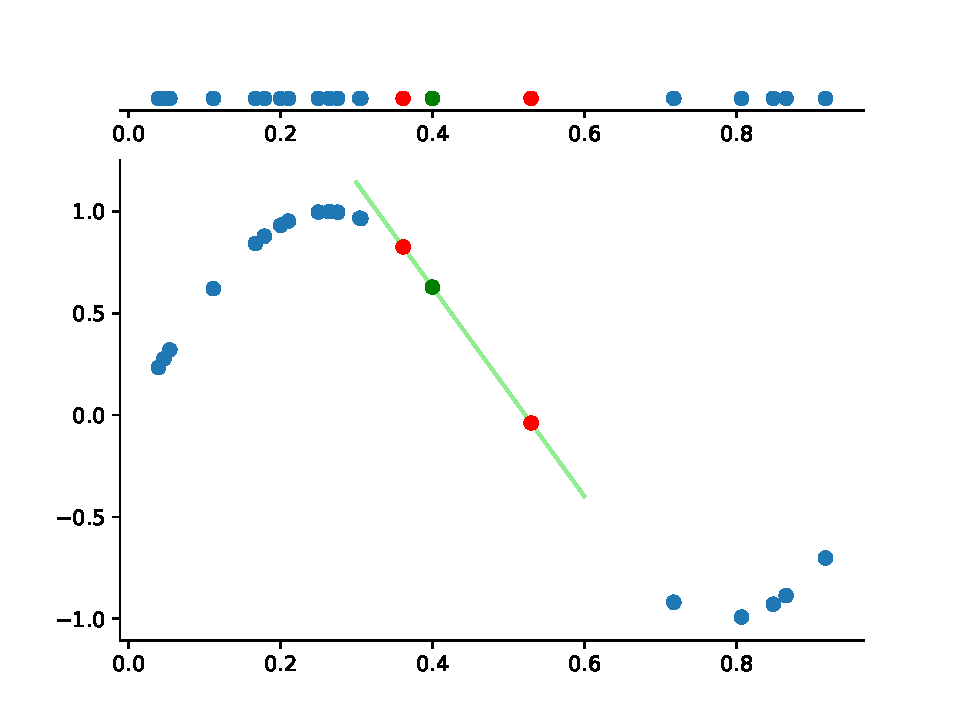
\includegraphics[width=0.8\linewidth]{images/vis1d.pdf}
	\caption{one-dimensional example of linear interpolation}
	\label{fig:one-dim-interpolation}
\end{figure}

In two dimensions things get more complicated as we now have a set of points with $X$ and $Y$ coordinates (Figure \ref{fig:3dinterpolate-1}). One fast way to find the closest points to the point that should be interpolated is using Delaunay triangulation. This separates the space between the points into triangles while trying to maximize their smallest angle. Afterwards the closest three points can be found very quickly by checking the nodes of the surrounding triangle  (Figure \ref{fig:3dinterpolate-2}).

\todo[inline]{It might be a better idea (and maybe more correct) to add the green point to the Delaunay list and use it's neighbors as the nearest points instead of the edges of the surrounding triangle.}

\begin{figure*}[h] % also temporary
	\centering
	\begin{subfigure}[t]{0.5\textwidth}
		\centering
		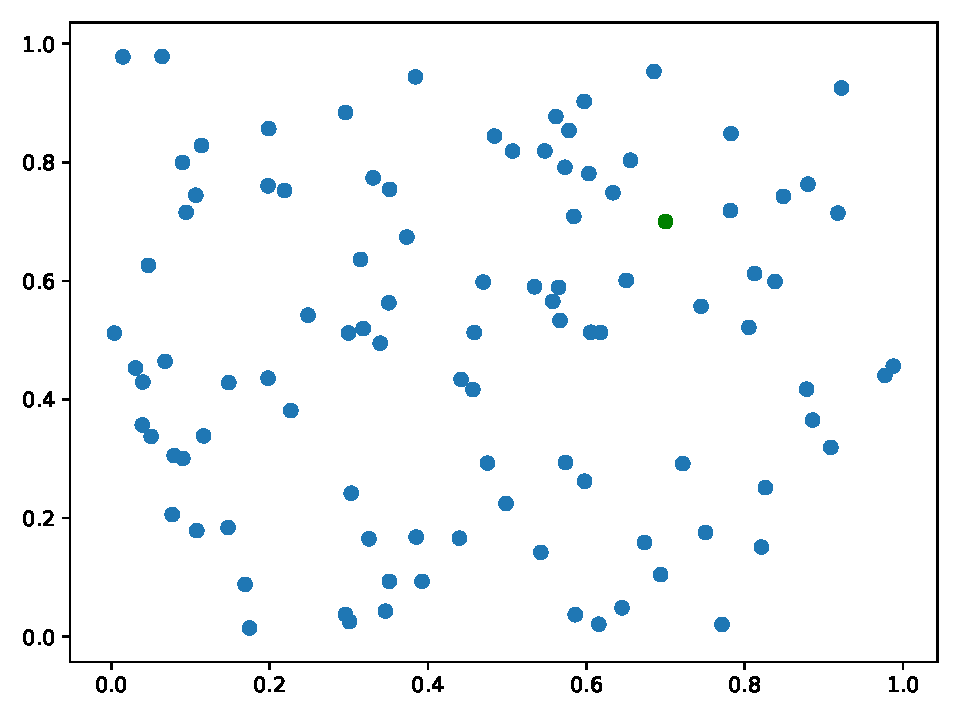
\includegraphics[width=\linewidth]{images/vis2d1.pdf}
		\caption{Lorem ipsum}
	\label{fig:3dinterpolate-1}
	\end{subfigure}%
	~ 
	\begin{subfigure}[t]{0.5\textwidth}
		\centering
		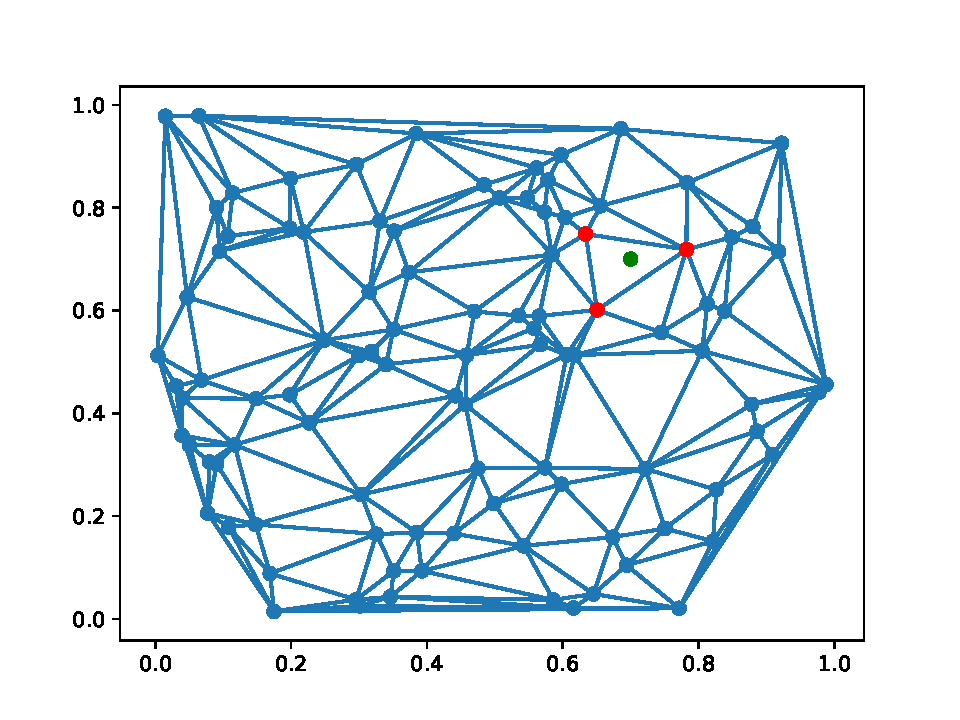
\includegraphics[width=\linewidth]{images/vis2d2.pdf}
		\caption{Lorem ipsum, lorem ipsum,Lorem ipsum, lorem ipsum,Lorem ipsum}
		\label{fig:3dinterpolate-2}
	\end{subfigure}
	\caption{Caption place holder}

\end{figure*}

\appendix
\chapter{Placeholder}

\lipsum[1]\footcite{Schaefer2016}\footcite{dvorakMoon}\footcite{MaindlSummary}\footcite{Burger2018}\footcite{Dorninger}\footcite{CollisionParameters}\footcite{CollisionTypes}

\printbibliography


\end{document}

